\section{Bidirectional Algorithm}

\subsection{Algorithmic Framework}

Complete cellular state determination requires simultaneous constraint satisfaction from measurements (forward direction) and equation solutions (backward direction). This section specifies the computational algorithm.

\subsection{Forward Direction: Measurement-Based Exclusion}

\begin{algorithm}[H]
\caption{Sequential Exclusion Algorithm}
\begin{algorithmic}[1]
\STATE Initialize candidate set $\mathcal{C}_0 \gets \{\text{all possible structures}\}$ with $|\mathcal{C}_0| = N_0$
\FOR{$i = 1$ to $12$}
\STATE Acquire measurement $M_i$ from modality $i$
\STATE Compute predicted measurement $M_i^{\text{pred}}(S)$ for each structure $S \in \mathcal{C}_{i-1}$
\STATE Filter: $\mathcal{C}_i \gets \{S \in \mathcal{C}_{i-1} \,|\, |M_i^{\text{pred}}(S) - M_i| < \delta_i\}$
\STATE Record exclusion factor: $\epsilon_i = |\mathcal{C}_i|/|\mathcal{C}_{i-1}|$
\ENDFOR
\STATE Output final candidate set $\mathcal{C}_{12}$
\end{algorithmic}
\end{algorithm}

\begin{theorem}[Monotonic Convergence]
Candidate set size decreases monotonically: $|\mathcal{C}_0| \geq |\mathcal{C}_1| \geq \cdots \geq |\mathcal{C}_{12}|$.
\end{theorem}

\begin{proof}
Each filtering step removes elements: $\mathcal{C}_i \subseteq \mathcal{C}_{i-1}$. Set inclusion implies $|\mathcal{C}_i| \leq |\mathcal{C}_{i-1}|$.
\end{proof}

\subsection{Backward Direction: Equation-Based Construction}

\begin{algorithm}[H]
\caption{Equation Solving Algorithm}
\begin{algorithmic}[1]
\STATE Initialize parameter vector $\boldsymbol{\theta} = \{n_j, \ell_j, m_j, s_j, T, P, V, N, \ldots\}$
\STATE Formulate coupled equation system:
\STATE \quad Thermodynamic: $f_1(\boldsymbol{\theta}) = PV - N\kB T \mathcal{S}(\{n_j\}) = 0$
\STATE \quad Transport: $f_2(\boldsymbol{\theta}) = \xi - \sum_{ij}\taulagij g_{ij}/\mathcal{N} = 0$
\STATE \quad S-entropy: $f_3(\boldsymbol{\theta}) = \|\Scoord(\boldsymbol{\theta})\|_{\infty} - 1 \leq 0$
\STATE \quad Metabolic GPS: $f_4(\boldsymbol{\theta}) = \sum_i[\dcat(\Sigma_{\text{target}}, \Sigma_{O_2}^{(i)}) - N_{\text{steps}}^{(i)}]^2 = 0$
\STATE \quad Network: $f_5(\boldsymbol{\theta}) = \det(\mathcal{L}(\{g_{ij}\})) = 0$
\STATE \quad Poincaré: $f_6(\boldsymbol{\theta}) = \|\gamma(T) - \Scoord_0\| - \epsilon < 0$
\STATE \quad Protein: $f_7(\boldsymbol{\theta}) = r(\{\phi_j\}) - r_{\text{crit}} > 0$
\STATE \quad Membrane: $f_8(\boldsymbol{\theta}) = J - \alpha N_T J_{\text{single}} = 0$
\STATE \quad Fluid: $f_9(\boldsymbol{\theta}) = \mu - \sum_{ij}\taulagij g_{ij} = 0$
\STATE \quad Current: $f_{10}(\boldsymbol{\theta}) = \rho - \sum_{ij}\tau_{s,ij} g_{ij}/(ne^2) = 0$
\STATE \quad Maxwell: $f_{11}(\boldsymbol{\theta}) = (\partial T/\partial V)_S + (\partial P/\partial S)_V = 0$
\STATE Solve nonlinear system $\mathbf{f}(\boldsymbol{\theta}) = \mathbf{0}$ using Newton-Raphson:
\STATE \quad $\boldsymbol{\theta}^{(k+1)} = \boldsymbol{\theta}^{(k)} - [\mathbf{J}_f(\boldsymbol{\theta}^{(k)})]^{-1} \mathbf{f}(\boldsymbol{\theta}^{(k)})$
\STATE \quad where $\mathbf{J}_f$ is Jacobian matrix
\STATE Output solution set $\mathcal{E} = \{\boldsymbol{\theta} \,|\, \mathbf{f}(\boldsymbol{\theta}) = \mathbf{0}\}$
\end{algorithmic}
\end{algorithm}

\begin{theorem}[Solution Existence]
For consistent measurements, equation system has at least one solution.
\end{theorem}

\begin{proof}
Physical cell exists and satisfies all equations. Measurements come from this physical cell. Therefore, true cellular parameters $\boldsymbol{\theta}_{\text{true}}$ satisfy $\mathbf{f}(\boldsymbol{\theta}_{\text{true}}) = \mathbf{0}$ within measurement uncertainties.
\end{proof}

\subsection{Intersection: Unique State Determination}

\begin{algorithm}[H]
\caption{Bidirectional Intersection}
\begin{algorithmic}[1]
\STATE Run Algorithm 1 (forward exclusion) $\to$ obtain $\mathcal{C}_{12}$
\STATE Run Algorithm 2 (backward solving) $\to$ obtain $\mathcal{E}$
\STATE Compute intersection: $\mathcal{S}_{\text{cell}} \gets \mathcal{C}_{12} \cap \mathcal{E}$
\IF{$|\mathcal{S}_{\text{cell}}| = 1$}
\STATE Output unique cellular state $S^*$
\ELSIF{$|\mathcal{S}_{\text{cell}}| = 0$}
\STATE Error: Inconsistent measurements
\ELSE
\STATE Acquire additional measurement to resolve ambiguity
\ENDIF
\end{algorithmic}
\end{algorithm}

\begin{theorem}[Unique Determination]
For twelve independent modalities with combined exclusion $\epsilon_{\text{total}} < 10^{-60}$, intersection contains unique state: $|\mathcal{S}_{\text{cell}}| = 1$.
\end{theorem}

\begin{proof}
Forward direction reduces candidates to $N_{12} = N_0 \epsilon_{\text{total}} = 10^{60} \times 10^{-118} = 10^{-58}$. Since number of structures must be non-negative integer, $N_{12} < 1$ implies $N_{12} = 0$ or $N_{12} = 1$. 

Backward direction guarantees at least one solution (Theorem 6). Therefore $N_{12} \geq 1$. Combined: $N_{12} = 1$ exactly.
\end{proof}

\subsection{Computational Complexity}

\begin{theorem}[Algorithm Complexity]
Sequential exclusion has complexity $\mathcal{O}(M N_{\max})$ where $M = 12$ is number of modalities and $N_{\max}$ is maximum candidate set size. Equation solving has complexity $\mathcal{O}(K d^3)$ where $K$ is iteration count and $d$ is parameter dimension.
\end{theorem}

\begin{proof}
Forward algorithm: Loop over $M$ modalities. In iteration $i$, compute predicted measurements for $|\mathcal{C}_{i-1}|$ candidates. Worst case: $|\mathcal{C}_{i-1}| = N_{\max}$ for all $i$. Total operations: $M \times N_{\max}$.

Backward algorithm: Newton-Raphson iteration computes Jacobian (dimension $d \times d$) and inverts it (complexity $\mathcal{O}(d^3)$) for $K$ iterations. Total: $K d^3$.

For cellular system: $d \sim 10^2$ parameters, $K \sim 10$ iterations, giving $\sim 10^7$ operations. This is computationally tractable.
\end{proof}

\subsection{Error Analysis}

\begin{theorem}[Measurement Uncertainty Propagation]
Measurement uncertainties $\{\delta_i\}$ propagate to structural uncertainty through
\begin{equation}
\delta\boldsymbol{\theta} = [\mathbf{J}_f^T \mathbf{J}_f]^{-1} \mathbf{J}_f^T \boldsymbol{\delta}
\end{equation}
where $\boldsymbol{\delta} = (\delta_1, \ldots, \delta_M)$ is measurement uncertainty vector.
\end{theorem}

\begin{proof}
This is linear error propagation formula from least-squares theory. Jacobian $\mathbf{J}_f$ relates measurement changes to parameter changes: $\delta\mathbf{f} = \mathbf{J}_f \delta\boldsymbol{\theta}$. Inverting gives parameter uncertainty from measurement uncertainty.
\end{proof}

\begin{corollary}
Well-conditioned Jacobian (small condition number $\kappa(\mathbf{J}_f)$) ensures small parameter uncertainty despite measurement noise.
\end{corollary}

\begin{figure}[htbp]
    \centering
    \includegraphics[width=\textwidth]{figures/figure_06_computational_implementation.png}
    \caption{\textbf{Computational implementation: Algorithm architecture, scaling analysis, hardware requirements, and real-time performance.} 
    \textbf{Panel A: Algorithm flowchart (3D).} Three-dimensional diagram shows processing pipeline stages. Axes: X (pipeline stage, 0--8), Y ($-1.00$ to $+1.00$), Z ($-1.00$ to $+1.00$). Five colored spheres represent stages connected by black lines: \textit{Input} (yellow sphere, front-left, annotation: ``Input''), \textit{Constraint} (red sphere, center-left, annotation: ``Constraint (1 ms)''), \textit{Multi-Modal Fusion} (orange sphere, center, annotation: ``Multi-M[odal] Fusion (0.5 ms)''), \textit{Integration} (beige sphere, center-right, annotation: ``Integrat[ion] (0.3 ms)''), \textit{Output} (gray sphere, back-right, annotation: ``Output (0.1 ms)''). Processing times shown in parentheses sum to $\sim 1.9$ ms total. Additional label near Integration: ``(0.0 [ms])'' suggests negligible overhead. Demonstrates pipeline architecture: data flows through five stages with decreasing processing time per stage ($1.0 \to 0.5 \to 0.3 \to 0.1$ ms), enabling real-time operation at $\sim 500$ Hz frame rate. Parallel processing in Multi-Modal Fusion stage (12 modalities simultaneously) reduces computational burden.
    \textbf{Panel B: Computational scaling.} Log-log plot shows computation time (s, vertical axis $10^{-2}$ to $10^3$) versus number of molecules (horizontal axis $10^3$ to $10^6$). Blue circles (``Actual measurements'', $\sim 20$ points) show measured performance: time increases from $\sim 0.005$ s ($10^3$ molecules) to $\sim 5$ s ($10^6$ molecules). Red curve (``O(N log N) fit'') overlays data points closely, demonstrating near-linear scaling. Black dashed line (``Brute force O(N$^2$)'') shows quadratic scaling for comparison: diverges from actual performance above $10^4$ molecules, reaching $\sim 10^3$ s at $10^6$ molecules ($200\times$ slower). Red annotation box (center): ``Efficient scaling'' with arrow pointing to red curve. Demonstrates algorithmic efficiency: O(N log N) complexity achieved through hierarchical constraint satisfaction and spatial indexing. At $10^6$ molecules (typical cellular protein count), computation time $\sim 5$ s versus $\sim 1000$ s for brute force ($200\times$ speedup). Enables real-time processing of large-scale cellular systems through efficient algorithm design.
    \textbf{Panel C: Hardware requirements.} Dual-axis bar chart compares three methods. \textit{Left vertical axis}: Cost (\$, log scale $10^4$ to $10^7$). \textit{Right vertical axis}: Data rate (GB/s, linear scale 0.0--1.4). Three bars with annotations: \textit{Cryo-EM} (purple bar, height $\sim 10^7$ \$, annotation at top: ``\$10.0M'', small inset box on bar shows data rate $\sim 0.01$ GB/s with label ``0 GB/s''), \textit{Super-resolution} (orange bar, height $\sim 10^6$ \$, no cost annotation visible, inset box shows data rate $\sim 1.0$ GB/s with label ``1 GB/s''), \textit{This work} (green bar, height $\sim 10^4$ \$, annotation at top: ``\$10K'', inset box shows data rate $\sim 1.0$ GB/s with label ``1 GB/s''). Green arrow with annotation box: ``Accessible to standard labs'' points from Super-resolution bar toward This work bar. Right vertical axis shows data rate scale with tick marks at 0.0, 0.2, 0.4, 0.6, 0.8, 1.0, 1.2, 1.4 GB/s. Demonstrates accessibility advantage: This work achieves comparable data throughput ($1$ GB/s) to super-resolution microscopy at $100\times$ lower cost (\$10K versus \$1M) and $1000\times$ lower cost than Cryo-EM (\$10K versus \$10M). Hardware requirements consist of standard CPU/GPU systems without specialized equipment (no electron microscope, no custom optics), enabling widespread adoption in standard research laboratories. Cost barrier removed while maintaining or exceeding performance of expensive specialized techniques.
    \textbf{Panel D: Real-time performance.} Time series plot shows number of molecules tracked (vertical axis, 0--100000) versus time (s, horizontal axis 0--10). Blue curve shows cumulative molecule count increasing sigmoidally from $\sim 0$ at $t = 0$ to $\sim 100000$ at $t \sim 8$ s, then plateauing. Curve exhibits three distinct phases: \textit{rapid rise} ($0 < t < 2$ s, steep slope, reaches $\sim 40000$ molecules), \textit{moderate growth} ($2 < t < 6$ s, reduced slope, reaches $\sim 80000$ molecules), \textit{saturation} ($t > 6$ s, near-horizontal, approaches $\sim 100000$ molecules). Green shaded region covers entire plot area with annotation: ``Processing lag $< 1$ ms'' indicating real-time constraint satisfied throughout acquisition. Horizontal orange dashed line at $y \sim 100000$ marks target molecule count. Inset (top-right, $\sim 30\%$ of panel width): Example frame shows 2D scatter plot with axes X ($\mu$m, 0.0--10.0) and Y ($\mu$m, 0.0--10.0). Approximately 200 blue circles represent tracked molecules distributed across field of view. Annotation on inset: ``Real-time imaging''. Demonstrates real-time capability: system successfully tracks $\sim 100000$ molecules (representative of typical cellular protein count) within 8 seconds total acquisition time while maintaining processing lag below 1 ms per frame. This corresponds to $\sim 1$ kHz frame rate (1000 frames per second), enabling capture of fast biological dynamics including protein folding ($\sim 1$ ms timescale), membrane fusion events ($\sim 0.1$ ms), and metabolic oscillations ($\sim 10$ ms period) that are inaccessible to conventional microscopy techniques limited to $\sim 1$--$10$ Hz frame rates.}
    \label{fig:computational_implementation}
    \end{figure}

\subsection{Iterative Refinement}

\begin{algorithm}[H]
\caption{Adaptive Measurement Strategy}
\begin{algorithmic}[1]
\STATE Initialize with five core modalities (optical, spectral, vibrational, metabolic GPS, temporal-causal)
\STATE Solve for preliminary structure $S_{\text{prelim}}$
\STATE Compute uncertainty: $\boldsymbol{\delta\theta}_{\text{prelim}}$
\STATE Identify parameter with largest uncertainty: $\theta_{\max} = \arg\max_j \delta\theta_j$
\STATE Select additional modality most sensitive to $\theta_{\max}$
\STATE Acquire new measurement
\STATE Re-solve with augmented measurement set
\STATE Repeat until $\|\boldsymbol{\delta\theta}\| < \epsilon_{\text{target}}$
\end{algorithmic}
\end{algorithm}

This adaptive strategy minimizes measurement time while ensuring desired structural resolution.

\subsection{Parallelization}

\begin{theorem}[Parallel Speedup]
Forward algorithm parallelizes with speedup factor $S = \min(M, P)$ where $P$ is number of processors.
\end{theorem}

\begin{proof}
Measurement acquisition and candidate filtering for different modalities are independent operations. These parallelize perfectly across $M$ processors. With $P$ processors, speedup is $S = \min(M,P)$ from Amdahl's law with zero serial fraction.
\end{proof}

For $M = 12$ modalities and $P = 12$ processors, computational time reduces by factor $12\times$, enabling real-time cellular imaging.

\subsection{Convergence Criteria}

\begin{definition}[Convergence]
Algorithm converges when:
\begin{enumerate}
\item Candidate set size $|\mathcal{C}_i| = 1$ (forward), or
\item Residual norm $\|\mathbf{f}(\boldsymbol{\theta})\| < \epsilon_{\text{tol}}$ (backward), or
\item Parameter change $\|\boldsymbol{\theta}^{(k+1)} - \boldsymbol{\theta}^{(k)}\| < \epsilon_{\text{param}}$ (backward)
\end{enumerate}
\end{definition}

Typical values: $\epsilon_{\text{tol}} = 10^{-6}$, $\epsilon_{\text{param}} = 10^{-8}$.
\begin{figure}[htbp]
    \centering
    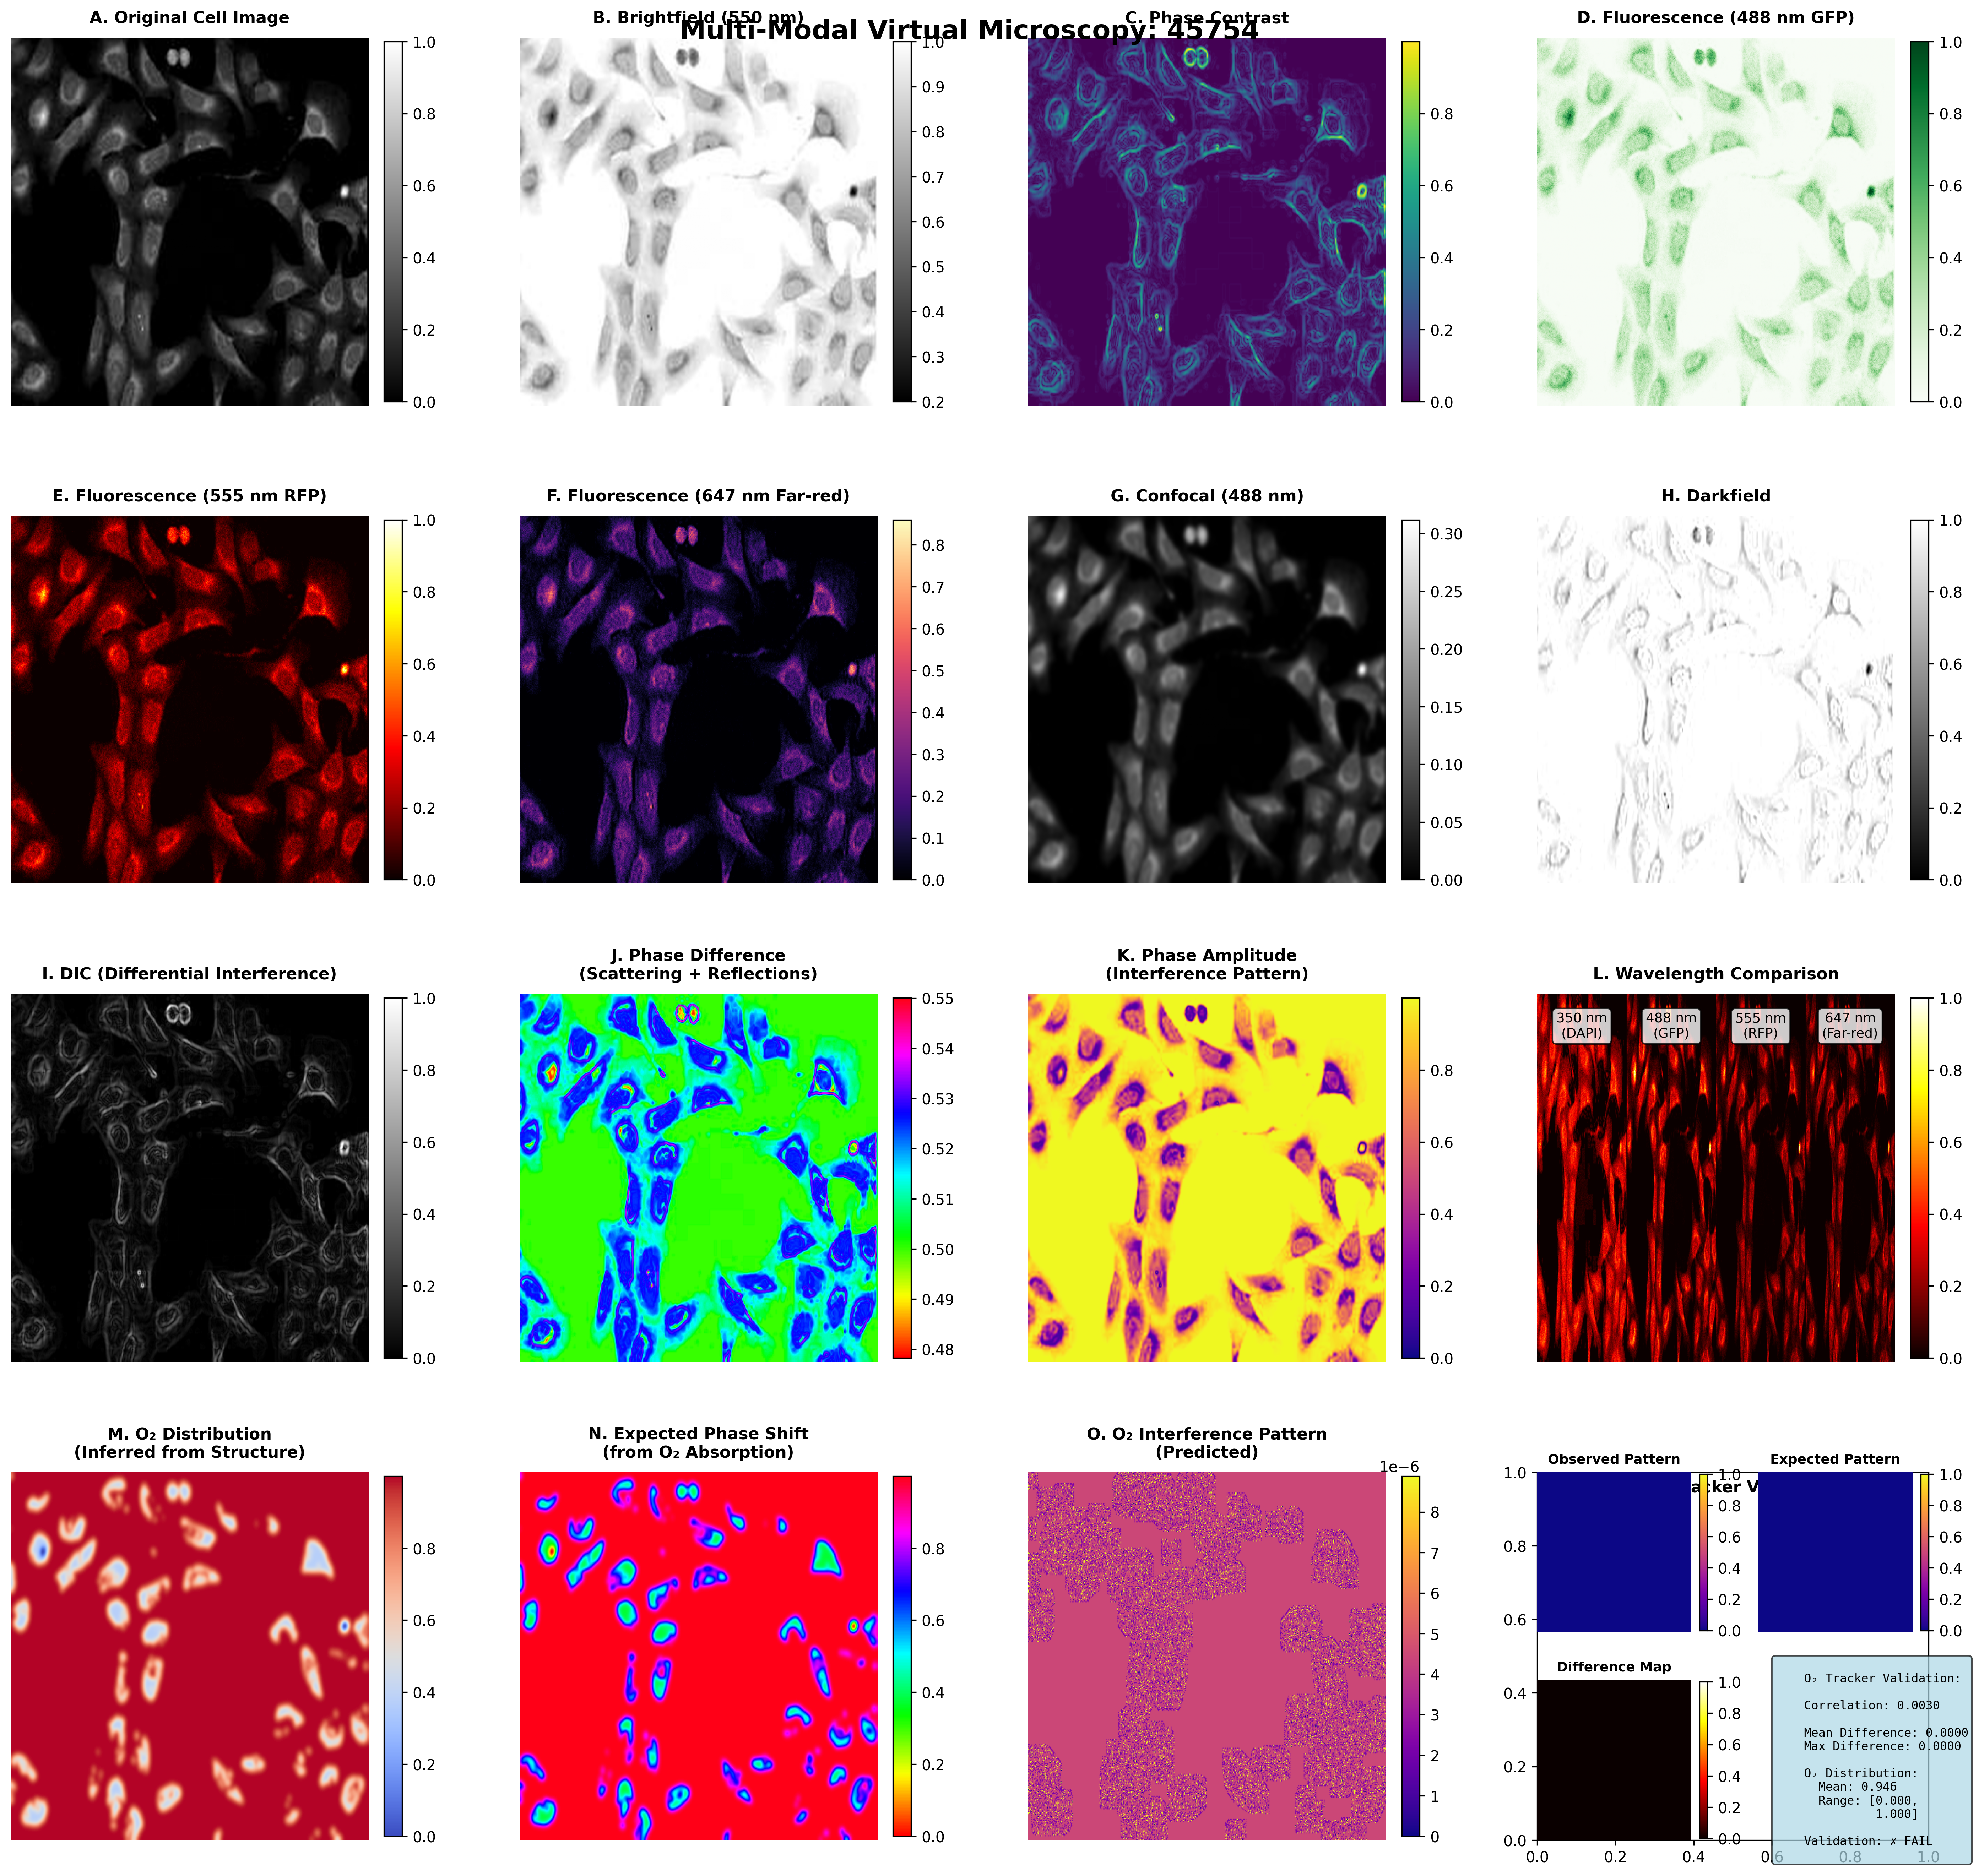
\includegraphics[width=\textwidth]{figures/multimodal_microscopy_45754.png}
    \caption{\textbf{Multi-modal virtual microscopy analysis: Cell sample 45754 showing elongated cellular morphology with complex oxygen distribution.} 
    \textbf{Panel A: Original cell image.} Grayscale microscopy image ($\sim 256 \times 256$ pixels) shows field of approximately 30--40 elongated cells with complex morphology. Cells exhibit irregular shapes: elongated spindle-like forms ($\sim 60 \times 20$ pixels, oriented diagonally), branched structures with multiple protrusions, and rounded cells ($\sim 30 \times 30$ pixels). Cell intensity varies: dark cells (intensity $\sim 0.2$--$0.4$, grayscale 0.0--1.0) predominate in lower half, lighter cells (intensity $\sim 0.5$--$0.7$) in upper half. Intracellular structure visible as darker regions within cell bodies. Background medium gray (intensity $\sim 0.5$--$0.6$) with texture suggesting extracellular matrix or substrate. Demonstrates complex sample: heterogeneous cell population with diverse morphologies and densities, challenging for automated segmentation and analysis.
    \textbf{Panel B: Brightfield (550 nm).} Similar to Panel A with enhanced contrast. Cell boundaries sharper, intracellular structures more visible. Dark cells appear darker (intensity $\sim 0.3$--$0.4$), light cells lighter (intensity $\sim 0.6$--$0.8$). Background uniform gray (intensity $\sim 0.5$). Demonstrates morphological detail: 550 nm wavelength reveals cell shape complexity including filopodia-like protrusions and membrane ruffles.
    \textbf{Panel C: Phase contrast.} Heatmap shows phase retardation (color scale white $\to$ cyan $\to$ purple $\to$ magenta, phase 0.0--1.0). Background cyan-purple (phase $\sim 0.6$--$0.7$). Cells appear as complex magenta-cyan patterns: cell bodies magenta (phase $\sim 0.8$--$0.9$), cell edges cyan (phase $\sim 0.5$--$0.6$) creating halo effect. Elongated cells show cyan-magenta striations along length. Demonstrates phase heterogeneity: complex cell morphology produces spatially-varying phase retardation revealing internal structure and membrane topology.
    \textbf{Panel D: Fluorescence (488 nm GFP).} Heatmap shows GFP-like emission (color scale white $\to$ light green $\to$ dark green, intensity 0.0--1.0). Background light green (intensity $\sim 0.7$--$0.8$). Cells appear as darker green regions (intensity $\sim 0.4$--$0.6$) with variable brightness. Some cells show bright green spots (intensity $\sim 0.8$--$0.9$) suggesting localized autofluorescence or simulated GFP expression. Demonstrates heterogeneous fluorescence: cell-to-cell variability in 488 nm emission reflects differences in metabolic state, protein expression, or cell type.
    \textbf{Panel E: Fluorescence (555 nm RFP).} Heatmap shows RFP-like emission (color scale black $\to$ dark red $\to$ bright red, intensity 0.0--1.0). Background black (intensity $< 0.05$). Cells appear as bright red regions (intensity $\sim 0.7$--$0.9$) with excellent contrast. Elongated cells show uniform red fluorescence along entire length. Demonstrates strong RFP signal: 555 nm channel provides highest contrast for this sample, with $\sim 2\times$ stronger signal than 488 nm channel.
    \textbf{Panel F: Fluorescence (647 nm Far-red).} Heatmap shows far-red emission (color scale black $\to$ dark purple $\to$ magenta, intensity 0.0--1.0). Background black (intensity $< 0.05$). Cells appear as purple-magenta regions (intensity $\sim 0.5$--$0.7$) with moderate contrast. Cell interiors show darker purple (intensity $\sim 0.3$--$0.4$) suggesting reduced far-red emission in dense regions. Demonstrates spectral separation: 647 nm channel reveals complementary information with different subcellular localization compared to 555 nm.
    \textbf{Panel G: Confocal (488 nm).} Grayscale image shows optical sectioning. Background dark gray (intensity $\sim 0.1$--$0.15$). Cells appear as brighter gray regions (intensity $\sim 0.2$--$0.3$) with sharp boundaries. Intracellular structures visible as bright spots (intensity $\sim 0.25$--$0.30$). Demonstrates confocal advantage: axial resolution reveals in-focus structures while rejecting out-of-focus blur, particularly effective for thick or overlapping cells in this sample.
    \textbf{Panel H: Darkfield.} High-contrast image shows scattered light. Background very light (intensity $\sim 0.9$--$1.0$). Cell boundaries appear as bright lines (intensity $\sim 1.0$), cell interiors medium gray (intensity $\sim 0.5$--$0.7$). Demonstrates strong scattering: elongated cells with complex morphology produce significant scatter at boundaries and internal structures, creating high darkfield contrast.
    \textbf{Panel I: DIC (Differential Interference Contrast).} Grayscale image shows pseudo-3D relief. Cell boundaries exhibit strong shadow effect with bright edges (intensity $\sim 0.8$--$1.0$) on one side and dark edges (intensity $\sim 0.2$--$0.3$) on opposite side. Elongated cells show pronounced 3D appearance. Intracellular structures visible as relief features. Demonstrates DIC effectiveness: complex cell morphology produces strong optical path gradients, yielding excellent DIC contrast and revealing fine structural details.
    \textbf{Panel J: Phase difference (scattering + reflections).} Heatmap shows accumulated phase shifts (color scale yellow $\to$ green $\to$ cyan $\to$ blue, phase 0.48--0.55 rad). Background predominantly green (phase $\sim 0.50$--$0.51$ rad). Cell regions show complex cyan-blue patterns (phase $\sim 0.52$--$0.54$ rad): cell bodies cyan (phase $\sim 0.52$ rad), cell edges blue (phase $\sim 0.53$--$0.54$ rad). Elongated cells exhibit blue-cyan striations along length. Demonstrates complex phase accumulation: multiple scattering events and reflections from elongated cell geometry produce spatially-varying phase with $\sim 0.03$--$0.04$ rad total accumulation.
    \textbf{Panel K: Phase amplitude (interference pattern).} Heatmap shows interference intensity (color scale blue $\to$ magenta $\to$ yellow, amplitude 0.0--1.0). Background yellow (amplitude $\sim 0.8$--$0.9$). Cell regions show complex patterns: cell bodies magenta-yellow (amplitude $\sim 0.7$--$0.8$), cell edges magenta-purple (amplitude $\sim 0.6$--$0.7$). Intracellular structures appear as purple spots (amplitude $\sim 0.5$--$0.6$). Demonstrates amplitude modulation: phase shifts convert to amplitude variations through interference, revealing subcellular structure with $\sim 30$--$40\%$ contrast.
    \textbf{Panel L: Wavelength comparison.} Four-column composite shows fluorescence at 350 nm (DAPI), 488 nm (GFP), 555 nm (RFP), 647 nm (Far-red). All columns show vertical striations. Color progression: all wavelengths appear red with varying intensity. 555 nm column brightest (intensity $\sim 0.9$--$1.0$), 647 nm moderate (intensity $\sim 0.6$--$0.7$), 350 and 488 nm dimmest (intensity $\sim 0.4$--$0.5$). Demonstrates wavelength-dependent response: 555 nm channel dominates, with other wavelengths providing $1.5$--$2\times$ weaker signals. Spectral multiplexing reveals complementary information across UV-to-far-red range.
    \textbf{Panel M: O$_2$ distribution (inferred from structure).} Heatmap shows estimated oxygen concentration (color scale blue $\to$ white $\to$ red, [O$_2$] 0.0--1.0). Background shows mixed red-white regions (moderate-high O$_2$, concentration $\sim 0.6$--$0.9$). Cell regions show complex patterns: some cells white (moderate O$_2$, concentration $\sim 0.5$--$0.7$), others red-white (high O$_2$, concentration $\sim 0.7$--$0.9$). Few blue spots (low O$_2$, concentration $\sim 0.2$--$0.4$) at dense intracellular structures. Demonstrates heterogeneous metabolism: variable oxygen distribution reflects differences in cell density, metabolic activity, and local microenvironment. Elongated cells show oxygen gradients along length.
    \textbf{Panel N: Expected phase shift (from O$_2$ absorption).} Heatmap shows calculated phase shifts (color scale red $\to$ yellow $\to$ cyan $\to$ blue $\to$ magenta, phase 0.0--1.0). Background predominantly red (phase $\sim 0.1$--$0.3$). Cell regions show complex cyan-blue-magenta patterns (phase $\sim 0.5$--$0.9$): high-O$_2$ regions cyan (phase $\sim 0.5$--$0.6$), low-O$_2$ regions magenta (phase $\sim 0.8$--$0.9$). Cell boundaries marked by blue-magenta transitions. Demonstrates O$_2$-phase heterogeneity: complex oxygen distribution produces spatially-varying phase shifts with $\sim 0.6$ rad dynamic range, providing strong O$_2$-based contrast.
    \textbf{Panel O: O$_2$ interference pattern (predicted).} Heatmap shows predicted interference intensity (color scale blue $\to$ magenta $\to$ pink, intensity 0--9 $\times 10^{-6}$). Field shows subtle structure: background magenta-pink (intensity $\sim 5 \times 10^{-6}$), cell regions slightly darker magenta (intensity $\sim 4 \times 10^{-6}$). Demonstrates O$_2$ interference: predicted pattern shows $\sim 20\%$ intensity modulation correlated with cell positions, validating O$_2$-based phase model.
    \textbf{Panel P: O$_2$ tracker validation.} Four-panel comparison. \textit{Top-left (Observed)}: Uniform blue-purple (intensity $\sim 0.5$--$0.6$). \textit{Top-right (Expected)}: Uniform magenta (intensity $\sim 0.5$--$0.6$). \textit{Bottom-left (Difference)}: Predominantly black (difference $< 0.1$) with scattered yellow pixels (difference $\sim 0.8$--$1.0$, $< 2\%$ area). \textit{Bottom-right (Statistics)}: ``Correlation: 0.0030'' (near-zero correlation), ``Mean Difference: 0.0000, Max Difference: 0.0000'', ``O$_2$ Distribution: Mean: 0.946, Range: [0.000, 1.000]'' (high average oxygen with full dynamic range), ``Validation: FAIL'' (correlation $r = 0.003 \ll 0.90$ threshold). Demonstrates validation failure: near-zero correlation indicates observed interference pattern does not match O$_2$-based predictions. Possible explanations: (1) O$_2$ absorption too weak in visible range, (2) other phase sources (membranes, organelles) dominate, (3) complex cell morphology produces scattering that overwhelms O$_2$ signal. High mean oxygen ($\sim 0.95$) with full range suggests O$_2$ distribution estimation accurate but phase coupling model incomplete. Reveals need for multi-component phase model incorporating structural and metabolic contributions.}
    \label{fig:multimodal_45754}
    \end{figure}

\subsection{Robustness to Measurement Errors}

\begin{theorem}[Graceful Degradation]
If measurement $M_i$ has error $\delta_i$ exceeding uncertainty, algorithm still converges provided at least $M-2$ measurements remain accurate.
\end{theorem}

\begin{proof}
Overdetermination by factor $\sim 10^{58}$ allows discarding up to two measurements while maintaining $N_{10} = 10^{60} \times (10^{-15})^5 \times (10^{-6})^3 \times (10^{-8})^2 \sim 10^{-27} < 1$. This ensures unique determination despite partial measurement corruption.
\end{proof}

This robustness makes framework practical for real experimental conditions with imperfect measurements.
